% ****** Start of file apssamp.tex ******
%
%   This file is part of the APS files in the REVTeX 4.1 distribution.
%   Version 4.1r of REVTeX, August 2010
%
%   Copyright (c) 2009, 2010 The American Physical Society.
%
%   See the REVTeX 4 README file for restrictions and more information.
%
% TeX'ing this file requires that you have AMS-LaTeX 2.0 installed
% as well as the rest of the prerequisites for REVTeX 4.1
%
% See the REVTeX 4 README file
% It also requires running BibTeX. The commands are as follows:
%
%  1)  latex apssamp.tex
%  2)  bibtex apssamp
%  3)  latex apssamp.tex
%  4)  latex apssamp.tex
%
\documentclass[%
 reprint,
%superscriptaddress,
%groupedaddress,
%unsortedaddress,
%runinaddress,
%frontmatterverbose, 
%preprint,
%showpacs,preprintnumbers,
%nofootinbib,
%nobibnotes,
%bibnotes,
 amsmath,amssymb,
 aps,
pra,
%prb,
%rmp,
%prstab,
%prstper,
floatfix,
]{revtex4-1}

\usepackage{physics}
\usepackage{graphicx}% Include figure files
\usepackage{dcolumn}% Align table columns on decimal point
\usepackage{bm}% bold math
\usepackage{chemformula}
\usepackage[flushleft]{threeparttable}
%\usepackage{hyperref}% add hypertext capabilities
%\usepackage[mathlines]{lineno}% Enable numbering of text and display math
%\linenumbers\relax % Commence numbering lines

%\usepackage[showframe,%Uncomment any one of the following lines to test 
%%scale=0.7, marginratio={1:1, 2:3}, ignoreall,% default settings
%%text={7in,10in},centering,
%%margin=1.5in,
%%total={6.5in,8.75in}, top=1.2in, left=0.9in, includefoot,
%%height=10in,a5paper,hmargin={3cm,0.8in},
%]{geometry}

\usepackage{../macros/mydefs}

\begin{document}

%\preprint{APS/123-QED}

\title{Applications of \ch{MoS2} as a Two-Dimensional Material Beyond Graphene}% Force line breaks with \\
%\thanks{Term paper for PHY 7050: Winter 2015}%

\author{Kraig Andrews}%
 \email{kraig.andrews@wayne.edu}
\affiliation{%
 Wayne State University Department of Physics and Astronomy%\\
}%

%\collaboration{MUSO Collaboration}%\noaffiliation


%\collaboration{CLEO Collaboration}%\noaffiliation

\date{\today}% It is always \today, today,
             %  but any date may be explicitly specified

\begin{abstract}
An article usually includes an abstract, a concise summary of the work
covered at length in the main body of the article. 
\end{abstract}

%\pacs{Valid PACS appear here}% PACS, the Physics and Astronomy
                             % Classification Scheme.
%\keywords{Suggested keywords}%Use showkeys class option if keyword
                              %display desired
\maketitle

\tableofcontents

\section{\label{sec:introduction} Introduction}

\section{\label{sec:graphene_properties} Graphene as a New Two-Dimensional Material}
\subsection{\label{subsec:discovery} The Discovery of Graphene}
By the end of the last century microelectronics had revolutionized the world, the majority which are silicon-based devices. Today, millions of these silicon-based devices are used in many common electronic devices and have become unavoidable throughout everyday life. Though the first field-effect device was patented in 1925, it was not until 1960 that the first metal-oxide semiconductor field effect transistor was demonstrated \cite{Lilienfeld1925, Atalla1960, Schulz1999}. A decade after the first device, devices were being made with several thousand components on a single chip. From there the progress increased at a rapid rate, a process now known as Moore's law, predicting that for each new generation of memory chip and microprocessor unit, the device size would be reduced by 33\%, the chip size would be increased by 50\%, and the number of components on a chip would quadruple every three years \cite{Schulz1999, Moore1965}. This proven to be true, and up until recently had shown no signs of stopping. Many times the material limitations were overcome by advances in technology that were seemingly insurmountable and effectively had placed a cap on Moore's law, which ultimately led to new techniques and even more pristine silicon-based materials. However, the limit to oxide thickness has finally placed a maximum on the growth of the silicon-based semiconductor device industy \cite{Schulz1999}. This impending limit caused many to look for solutions that involved the use of \ch{SiO2} devices and also alternatives to silicon. The result of the latter has given way to a breadth of literature and research that was unforseen a decade before. The search for alternatives to silicon resulted in research into many new, nontraditional materials. Several notable examples are organic conductors and carbon nanotubes \cite{Mascaro2001, Baughman2002}. Arguably one of the most interesting nontraditional materials to come out of such research was graphene.  
\\ \\

In 1985, with the discovery of fullerenes the amount of known carbon allotropes increased \cite{krotoFullerenes1985, nanoscaleReview2011}. Fullerenes suggested the existence of a one-dimensional form of carbon, known as carbon nanotubes, which were first demonstrated in 1991 \cite{iijimaCarbonNanotubes1991}. Despite several theoretical studies involving the use of a single layer of graphite, it was not until 2004 that the first monolayer graphene sheet was isolated \cite{novoselovEtAl2004, novoselovEtAl2005}. In the most basic sense, graphene is simply a single layer of carbon atoms densely packed into a honeycomb lattice. It is used to describe properties several carbon-based materials (graphite, fullerenes, nanotubes, etc..., see Fig.\ref{fig:sp2}) \cite{Dresselhaus2002, Brenner2002, novoselovEtAl2004}. This was significant because scientists had tried for many years to synthesize monolayers of graphite, though only succeeding in obtaining materials around 10 layers thick \cite{nanoscaleReview2011}.


\begin{figure}
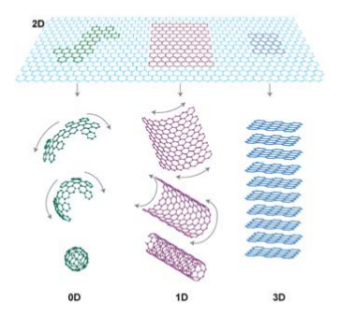
\includegraphics[height=5cm, width=5cm]{../figs/multiDimGraphene}
\caption{Graphene can be envisioned in several dimensions. 0-dimensional buckyballs, 1-dimensional nanotubes, or 3-dimensional graphite \cite{Novoselov2007}.}
\label{fig:sp2}
\end{figure}



\begin{figure}
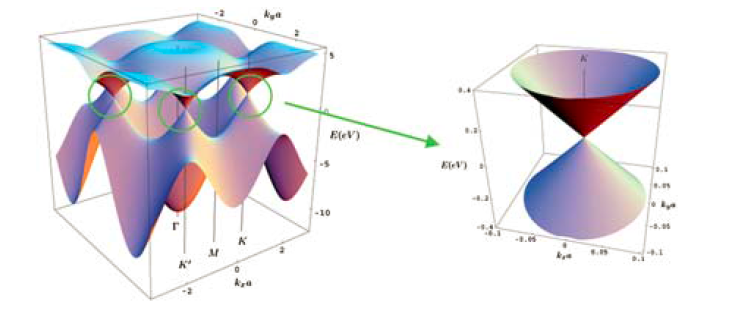
\includegraphics[height=3cm, width=6cm]{../figs/grapheneBandGap}
\caption{3D representation of the electronic band structure of graphene. The right side shows an enlarged view near the Fermi level in one $k$ point \cite{nanoscaleReview2011}.}
\label{fig:grapheneBands}
\end{figure}


\subsection{\label{subsec:properties_graphene} Properties of Graphene}
To date, graphene's properties have been the focus of much research both theoretical and experimental. Graphene has many unique properties that have paved the way for new subfields in condensed matter physics (i.e. 'relativistic' condensed matter physics). These properties are primarily a result of its low dimensionality and its band structure that allow electrons to mimic relativistic particles \cite{Giem2007}. This newly discovered phenomenon has allowed for the study of relativistic effects in condensed matter experiements. This includes the appearance of the atypical quantum Hall effect and the confirmation of other relativistic phonomena \cite{Geim2005_quantum, Zhang2011, Williams2007}. However, it is worth noting that this peculiar band structure can be modified by stacking three or more layers of graphene \cite{nanoscaleReview2011}. 
\\ \\
For applications to electronics a material's band gap is of interest. In graphne, however, the conduction and valence bands touch at a single point as shown in fig. \ref{fig:grapheneBands} \cite{Wallace1947, nanoscaleReview2011}. As a result graphene has no band gap (small band gaps of a few hundred $\textrm{MeV}$ can be introduced in bilayer graphene) \cite{grapheneLike2Dreview2013}. The absence of a band gap is also interesting in the context of the material's optical properties and the implications of these. The absence of a band gap allows for the absorption of light over a large range of the electromagnetic spectrum, ranging from infrared ($< 1.65 \mathrm{\,eV}$) to ultraviolet ($> 3.2 \mathrm{\,eV}$) giving potential for electronic-photonic device applications \cite{Wang2008, Geim2011, Xia2009}.  
\\ \\
Graphene's mechanical properties have been of much interest over the last decade. Graphene has a Young's modulus of $\sim 1000 \mathrm{\,GPa}$ with a breaking stength that is 13\% of that \cite{Bertolazzi2011, 2DflexibleNanoElectronics2014}. It can also sustain elastic deformations of 20\% and due to its two-dimensional nature it has a high pliability \cite{nanoscaleReview2011}. Mechanically, graphene is an exciting material due to the fact that it lies in the extreme ranges of some metrics considering its size and dimensionality. 
\\ \\
The mobility in graphene is another property that initially made the material so appealing (and still quite appealing to some degree). Graphene's mobility is about 1000 times that of silicon's \cite{Dargys1994, 2DflexibleNanoElectronics2014}. The outstanding crystal quality in larges scale (a few microns) is the major contributing factor here. Without many defects or imperfections the electrons can travel long distances, as much as several micrometers, without being scattered even on rough substrates \cite{nanoscaleReview2011, Du2008}. The average electron mobility obtained in graphene varies depending on temperature, but the most commonly measured value is $\mu = 100,000\mathrm{\,cm}^2\mathrm{V}^{-1}\mathrm{s}^{-1}$ with values up to $\mu = 500,000\mathrm{\,cm}^2\mathrm{V}^{-1}\mathrm{s}^{-1}$ obtainable at low temperatures \cite{vanderWaalsHeterostruct2013}.


\section{\label{sec:TMDs} Transition Metal Dichalcogenides}
Graphene is being studied for its unique porperties, however, many other two-dimensional materials are known. Some of the two-dimensional materials being studied in addition to graphene are known as transition metal dichalcogenides (TMDs) \cite{Mattheiss1973, Wilson1969}. TMDs consist of hexagonal layers of metal atoms (M) in between two layers of chalcogen atoms (X) such that the stoichiometry of the material is \ch{MX2} \cite{grapheneLike2Dreview2013}. The material is dependent on the combination of transition metal, typically one of: \ch{Mo}, \ch{W}, \ch{Nb}, \ch{Re}, \ch{Ni}, or \ch{V}, and chalcogen, typically one of: \ch{S}, \ch{Se}, or \ch{Te} \cite{Wilson1969}. These materials are commonly are stacked together which involves van der Waals interactions between adjacent sheets and covalent bonding within each individual sheet (see fig. \ref{fig:mos2diagram}) \cite{grapheneLike2Dreview2013}. There are wide variety of properties exhibited by these structures, which include insulator or metal. In addition, they can also display some interesting properties like the topological insulator effect, superconductivity, and thermoelectricity \cite{Lang2012, Zhang2012, Gamble1975, Xie2009}. Ongoing research also includes graphene-like nano materials like silicene and germanene, which are the silicon and germanium-based versions of graphene and are found to show properties that are similar to graphene \cite{Takeda1994, Cahangirov2009}. These two-dimensional materials are becoming increasingly attractive for a wide-range of applications due to their distinct properties. 
\begin{figure}
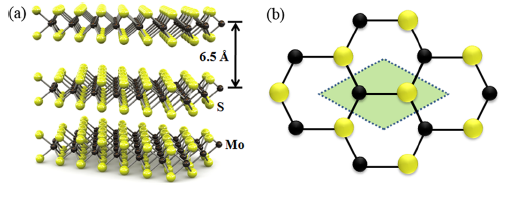
\includegraphics[height=3cm, width=7cm]{../figs/mos2diagram}
\caption{(a) The atomic structure of layered \ch{MoS2}. Different sheets are composed of three atomic layers \ch{S}-\ch{Mo}-\ch{S}, where \ch{Mo} and \ch{S} are covalently bonded \cite{Kis2011, grapheneLike2Dreview2013}. (b) Top view of the honeycomb lattice \cite{grapheneLike2Dreview2013}.}
\label{fig:mos2diagram}
\end{figure}

\subsection{\label{subsec:mos2_properties} Properties of \ch{MoS2}}
As discussed in sec. \ref{subsec:properties_graphene}, pristine graphene has no band gap. Though it is possible introduce a band gap in bilayer graphene and graphene nanoribbions, the appeal of many TMDs is that they have direct band gaps which make them ideal candidates for electronic material applications \cite{grapheneLike2Dreview2013}. One such example of a semiconducting TMD is \ch{MoS2} (molybdenum disulphide). TMDs, and more specifically \ch{MoS2} and the properties it exhibits have been studided to some extent for several decades with electrical measurements dating back to the 1960s \cite{Frindt1963, Fivaz1967}. However, as of late there has been renewed interest in several TMDs are their potential applications. 
\\ \\
Like graphene, and many other 2D materials, \ch{MoS2} has a Young's modulus that is comparable to steel ($\sim 205 \mathrm{\,GPa}$) \cite{Warlimont2009}. The Young's modulus of single-layer \ch{MoS2} is $\sim 270 \mathrm{\,GPa}$. The Young's modulus of bulk \ch{MoS2} is $\sim 240 \mathrm{\,GPa}$. The fact that monolayer \ch{MoS2} has a higher Young's modulus than its bulk material counterpart is thought to be mostly due to defects in the material, interlayer sliding, or the absence of stacking faults in monolayer samples \cite{Lembke2015}. In a further study it was found that the Young's modulus of multilayer \ch{MoS2} ranging in thickness from 5 to 25 layers was $330 \pm 70 \mathrm{\,GPa}$ \cite{Castellanos2012}. In addition, both single and bilayer \ch{MoS2} have a breaking strength of about 6\% and 11\% of their Young's modulus, respectively \cite{Bertolazzi2011}. This is an indication that \ch{MoS2} is quite flexible compared to other commonly used engineering materials (stainless steel $\sim 0.4\%$, kevlar $\sim 2.6\%$) \cite{Gere1997}. 
\\ \\
As stated before, what \ch{MoS2} and some other TMDs appealing for applications, specifically for use in integrated circuits and logic applications (see sec.\ref{sec:mos2_applications} for more on applications). Monolayer \ch{MoS2} has an indirect band gap of $1.8 \mathrm{\,eV}$ and few layer (bulk) \ch{MoS2} has a direct band gap of $1.3 \mathrm{\,eV}$ \cite{grapheneLike2Dreview2013, Kam1982, Mak2010, Gourmelon1997, Fortin1982}. This change in transition from an indirect band gap semiconductor to a direct band gap semiconductor is shown in fig.\ref{fig:mos2bandgap}.
\begin{figure}
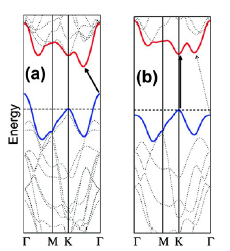
\includegraphics[height=4.5cm, width=3.75cm]{../figs/mos2bandgap}
\caption{Calculated band structures of bulk (a) and monolayer (b) \ch{MoS2} and the arrows indicate the lowest energy transition \cite{Splendiani2010}.}
\label{fig:mos2bandgap}
\end{figure}
The unusual electronic structure of mono and few-layer \ch{MoS2} which ultimately results in some unique optical properties are due to the composition of the material's conduction and valence bands. The valence band maximum at the $\Gamma$ point shifts downward to the $K$ point of the Brillouin zone as the number of layers decreases \cite{Mak2010, Splendiani2010}. The change in the band structure as a function of the amount of layers is due to quantum confinement and the change in hybridization between $p_z$ orbitals on \ch{S} atoms and $d$ orbitals on \ch{Mo} atoms \cite{Li2007, Mak2010, Splendiani2010}. Using quantum mechanical modeling systems to investigate the many-body electronic structure of \ch{MoS2} (density functional theory) it has been shown that the conduction band states at the $K$ point are primarly the result of $d$-orbital electrons localized on the \ch{Mo} atoms in between layers and are relatively unaffected by interlayer coupling \cite{Kohn1964, Wang2012a}. Conversely, states near the $\Gamma$-point are strongly affected by interlayer coupling due to the effects of antibonding $p_z$-orbitals on the \ch{S} atoms and the $d$ orbitals on the \ch{Mo} atoms \cite{Splendiani2010}. The result of this is that the states near the $K$-point are, for the most part, unchanged while the states near the $\Gamma$-point are shifted causing the change from an indirect to a direct band gap as the amount of layers of the material is decreased. 
\\ \\
Carrier mobility in two-dimensional TMDs are affected by scattering. The amount by which the scattering affects the mobility is dependent on a number of factors, namely: material thickness, carrier density, effective mass, temperature, and electronic and phonon band strucutre \cite{Wang2012a}. The main sources of scattering in 2D TMDs are: acoustic and opitcal phonon scattering and Coulomb scattering \cite{Ando1982, Ridley1982}. 

\section{\label{sec:synthesis_methods} Mechanical Exfoliation and Characterization of \ch{MoS2} Nanosheets}
There exist several methods that can be used to prepare atomically thin nanosheets of \ch{MoS2} (and other TMDs). Among these several methods are mechanical exfoliation, chemical exfoliation, chemical vapor deposition, and sonication \cite{grapheneLike2Dreview2013}. The method of mechanical exfoliation used to synthesize monolayer and few-layer \ch{MoS2} is very similar to the method use by Geim et al. to synthesize their samples of graphene from 3D graphite \cite{novoselovEtAl2005}. 
\\ \\
To date, mechanical exfoliation remains the best method to synthesize \ch{MoS2} crystals of the highest quality. The process involves taking bulk \ch{MoS2} crystals and peeling thin layers from the bulk material using some adhesive material. Commonly, the adhesive material is Scotch tape, though there have been variations on this such as a silicone stamp, instead \cite{Gomez2010}. This leaves a number of flakes attached to the surface of the adhesive. The flakes that are attached to the adhesive are then placed onto a substrate using instruments like plastic tweezers to further separate the flakes from the adhesive material. The process results in mono and few-layer flakes of \ch{MoS2} being deposited on the substrate \cite{Li2014}. In addition to mono and few-layer flakes of \ch{MoS2} being deposited on the substrate, the most common substrate being \ch{SiO2}/\ch{Si}, a quantity of thicker flakes of \ch{MoS2} are deposited as well \cite{acsnanoReview2013}. This is demonstrated in fig.\ref{fig:exfoliation}, showing the varying thicknesses of \ch{MoS2} flakes on a substrate. As a result a method is needed to further differentiate between the flakes of varying thicknesses on that have been deposited on the substrate before any type of fundamental research can be done on the material. \\ \\
\begin{figure}
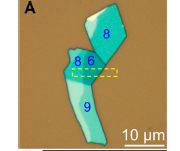
\includegraphics[height=4.5cm, width=4.5cm]{../figs/exfoliation}
\caption{Color image of a \ch{MoS2} deposited on a $90 \mathrm{\,nm}$ \ch{SiO2}/\ch{Si} substrate. The digits indicate the layer numbers of \ch{MoS2} nanosheets \cite{Li2014}}.
\label{fig:exfoliation}
\end{figure}
Determing the size synthesized two-dimensional materials is inherently challenging due to the small sample sizes. Several methods have been developed throughout the years to indentify and characterize these materials. The method used is dependent on the desired properties of the material that are of interest. For locating and subsequently determining the thickness of \ch{MoS2} optical microscopy is one techinique that does well to identify single and multi-layer flakes \cite{acsnanoReview2013}. In addition, to identify the thickness of these flakes, a common technique involves the use of atomic force microscopy (AFM).

\section{\label{sec:mos2_applications} Applications of \ch{MoS2}}

\section{\label{sec:state_of_the_art} State of the Art}

\section{\label{sec:problems_and_outlook} Problems and Outlook}


\bibliographystyle{plain}
\bibliography{../bibs/refs}
\end{document}
%
% ****** End of file apssamp.tex ******

